
\chapter{手机主题推荐系统整体设计与实现}
    \section{引言}
    小米主题应用拥有成千上万款主题包,而一个用户整个活跃周期只能接触不到十分之一的主题,所以我们现在面临的一个问题是,如何帮助用户发现新的主题,这些主题同时满足俩个条件:1、不能和用户之前看过的、购买过的主题包重复。2、不能和用户之看买过的、购买过的主题不相关,而这也是我们开发的手机主题推荐系统所要达到的目标之一。除此之外,手机主题推荐系统要达到的目标包括帮助第三方设计师推广其作品。手机主题应用本身既不生产主题包,也不消费主题包,存在的价值就在于提供一个平台,能让用户、设计师和广告商从中受益。每个设计师都希望更多的用户体验、使用他们的主题。得益于个性化推荐系统的投入使用,我们现在可以把更多的主题包直接推送给那些潜在消费者面前。

    本章节主要介绍手机主题推荐系统的完整架构。如\autoref{pic:construct}可知推荐引擎主要由推荐模块、用户画像模型、用户兴趣探索模块组成。
    \section{手机主题推荐系统设计}
    
    \begin{figure}
      \centering
        \framebox{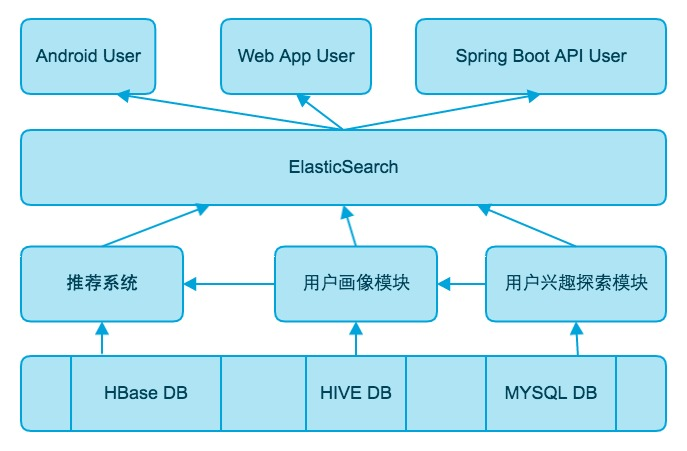
\includegraphics[scale=0.6]{figures/construct}}
        \figcaption{推荐系统引擎框架总览图}
        \label{pic:construct}
    \end{figure}

    推荐系统框架如\autoref{pic:construct}。最顶层显示的是推荐系统对外服务的客户端。由于不同展位的输入输出参数差异较大,因此这一层没有做过多的抽象,每个展位有自己特定的接口Json定义,接口层通过调用ElasticSearch搜索服务引擎实现秒级别的用户推荐结果列表。推荐系统利用离线方式更新ElasticSearch搜索服务器数据。用户画像模块除了作为推荐系统的输入数据外,也可以直接作为ElasticSearch的输入。用户兴趣探索模块定期扫描活跃用户和上架主题包,通过分析用户行为日志更新用户画像。从接口层接受到的每次响应请求会被记录成用户行为数据,包括请求的一些必要的上下文信息以及用户及主题包的特征信息。借助HBase、Hive、Mysql等数据平台对原始日志进行处理,从而得到需要的各种数据及模型:包括用户的画像信息,用户之间的相似度,商品之间的相似度。在推荐系统的候选集生成这一块,重度使用了item-based协同过滤算法,而对于那些行为稀少的用户和新用户,需要根据平台的特点进行做好冷启动策略。
    对于Spring Boot API 输入、输出数据格式分别如\autoref{code:api_input}和\autoref{code:api_output}。\\\\
    \begin{lstlisting}[language=json,firstnumber=1,label={code:api_input}, caption={Spring Boot API 输入格式}]
      {
        "user_id":"123",
        "dims":{"type":"normal", "free_or_charge":"mixed"},
        "white_list":{"id":1141},
        "max_number":"8",
        "start_date":"2016-07-01,
        "end_date":"2016-08-01
      }
    \end{lstlisting}

    \begin{lstlisting}[language=json,firstnumber=1,label={code:api_output}, caption={Spring Boot API 输出格式}]
    {
      "code":0,
      "message":"successfully",
      "data":{
        "total":111,
        "themes":[{
          "id":1141,
          "subscribe":1,
          "business":null,
          "keytype":"market:orderid",
          "tag":null,
          "name":"lovely baby",
          "displayName":"小可爱",
          "description":"家庭,儿童欢乐多",
          "author":"摆渡车1024",
          "sigModel":2,
          "type":2,
          "dependency":null,
          "createTime":1462447261000,
          "dims":null}
        ]}
    }
    \end{lstlisting}

    \subsection{数据采集和日志格式化}
    我们的数据采集来源包括移动端埋点和用户请求。目前常见的前端埋点技术有三类:代码触发埋点、可视化触发埋点和延迟埋点,根据手机主题商店的业务特点和用户规模,我们选用可视化触发埋点,当用户在UI上点击了某个可埋点的控件时,会自动触发回调函数调用接口发送相应事件的log信息,可视化触发埋点不同于代码触发埋点,其理念是把核心代码和配置、资源分开,在APP启动的时候通过网络更新配置和资源即可,不必每一个埋点都需要写代码,埋点产生的数据量很少,且只针对特定人群,所以用来做A/B测试的数据源。用户关键行为会被上传、存储到服务器。获取数据后根据数据来源和存储方式,将日志格式化为:public日志、nginx日志、binlog日志和passport日志,public日志存放手机端用户请求log,nginx日志存放Web端用户请求,binlog日志是将public日志同步到NoSQL DB的数据,passport日志存储用户验证信息等数据。

    \subsection{用户画像的收集}
    当上述日志格式化生成,通过每日定时任务扫描passport日志就可以获取新注册用户并为其在ElasticSearch创建一个topic,同时利用移动端埋点功能获取到用户手机IMEI号、经纬度等基本信息,利用用户注册手机号或者邮箱账号获取用户的通信录和好友信息,借助好友信息完善此用户的用户画像,除此之外有时可以借助第三方接口获取用户的基本信息。

    \subsection{商品标签的构建}
    小米手机主题应用商店里的主题包大多数是由第三方设计师创建、当设计师上传成品到官方产品库时会被要求填写作品标签,官方审核员也会更改、删除、添加一些标签,作品上架后用户在浏览、购买时产生的评论文本也会生成一些标签,商品标签的构建也只涉及到标签生成,没有产生权重。

    \subsection{候选集的生成}
    通过用户与商品的交互行为矩阵,我们最终得到了带有标签权重的候选集,具体算法是利用Item-based协同过滤算法生成候选集,定义N$_u$表示用户u之前喜欢的主题集合,则用户u对主题i的偏好度根据\autoref{ItemCF}可计算得到。
    \begin{equation}
    p(u,i)=\sum \limits _{j\in N(u)}^{} r(u,j)s(i,j)
    \label{ItemCF}
    \end{equation}

    其中,r$_{u,j}$表示用户u对主题j的偏好度,s$_{i,j}$表示主题i和主题j之间的相似度。Item-based协同过滤算法定义俩个主题之间的相似度由集中在这个俩个主题的用户行为数据计算得出。N$_{i}$为看过主题i的用户集合,N$_{j}$为为看过主题j的用户集合,因此,主题i和主题j的相似度计算公式为\autoref{Item-item-similar}。
    \begin{equation}
    s(i,j)=\frac{\left | N(i)\cap N(j) \right |}{\sqrt{\left | N(i) \parallel N(j) \right |}}
    \label{Item-item-similar}
    \end{equation}

    根据\autoref{Item-item-similar}可知,如果有很多用户同时看了主题i和主题j,那么主题i和主题j之间的相似度就会很高,不幸的是,这也会导致所有热门主题之间的相似度都很高,导致推荐结果包含热门主题包过多。我们的解决思路是对热门主题包降权,同时控制热门主题所占比例。

    \subsection{排序}
    排序主要是对候选集的生成的标签权重做排序,但会加入一些倾斜因子,如用户活跃度、主题包的热度、经纬度等因子,最终根据标签权重+倾斜因子的排序得到推荐结果。

  \section{用户画像与用户兴趣探索}
  众所周知用户的需求是动态变化着的,不管是随着季节周期性变动,还是随着年龄发生非逆转变化,都意味着一些标签需要删除掉,一些标签需要加进来。用户画像的数据来源包括:原始的用户行为数据和用户兴趣探索模块,前者只是更新那些显而易见的标签,而后者负责在海量数据中挖掘出那些稍纵即逝的用户行为并准确分析用户的意图,而用户兴趣探索对活跃用户效果相对较好,并且针对小众主题包进行挖掘的效果很棒,可以明显提升推荐结果的多样性。除此之外,我们利用基于时间窗口的遗忘机制解决了新、旧用户兴趣的融合问题,时间窗口机制与自然遗忘规律相似,排前面的标签时效性最好,排后面的标签时效性差,将会被优先淘汰。通过设置时间窗口的大小、时间窗口的滑动速率,可以间接控制新、旧兴趣的比例。

  \section{用户画像与推荐系统}
  一个推荐系统要给用户提供个性化的、高效的和准确的推荐,则意味着推荐系统应能够获取反映用户多方面的、动态变化的兴趣偏好,推荐系统有必要为用户建立一个用户兴趣探索模型,该模型能获取、表示、存储和修改用户兴趣偏好,能进行推理,对用户进行分类和识别,帮助系统更好地理解用户特征和类别,这就是我们要引进用户画像的根本原因。用户画像模块和兴趣探索模块的关系如\autoref{pic:hl_iterate}所示。
  \begin{figure}
    \centering
      \framebox{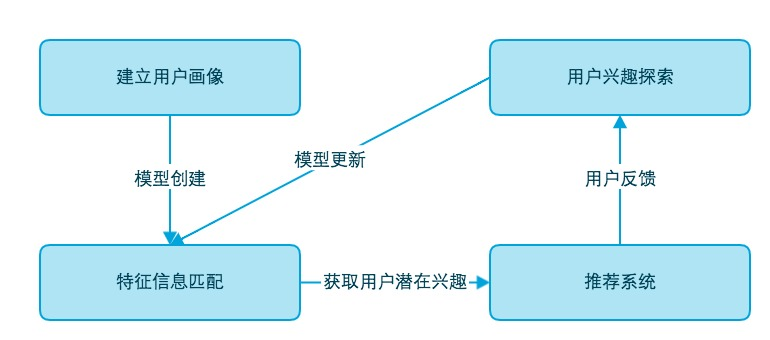
\includegraphics[scale=0.4]{figures/hl_iterate}}
      \figcaption{用户画像数据流图}
      \label{pic:hl_iterate}
  \end{figure}

  一个好的用户画像需要有一个完整的标签体系,包括标签的数量、质量和粒度。其中标签的数量直接影响推荐系统的结果完整度,标签的质量直接影响推荐系统的精度,而标签的粒度会影响推荐系统的用户满意度。完善的标签体系更像一个金字塔,一级是最基本的概念标签,如动漫、运动等,数量被控制在几十个左右,二级标签是上层标签的扩展,如美少女动漫、搞笑动漫、篮球运动、足球运动,三级标签就是指具体化了的标签,如街头篮球、NBA篮球、CBA篮球等。对于活跃度高的用户标签倾向于下沉,推荐结果数据多、精度高,活跃度低的用户反之。对于一个新创建的用户画像,刚开始只包含最基本的用户人口信息,随着用户行为数据的累积会逐渐丰富起来。

  \section{本章小结}
  本章首先介绍了整个推荐系统结构,然后介绍了数据集的生成、格式,以及基于数据集的用户画像建模和商品标签建模,最后介绍了用户画像和用户兴趣探索,用户画像和推荐系统的依赖关系。